\begin{frame}
    \frametitle{Game - Definition}

    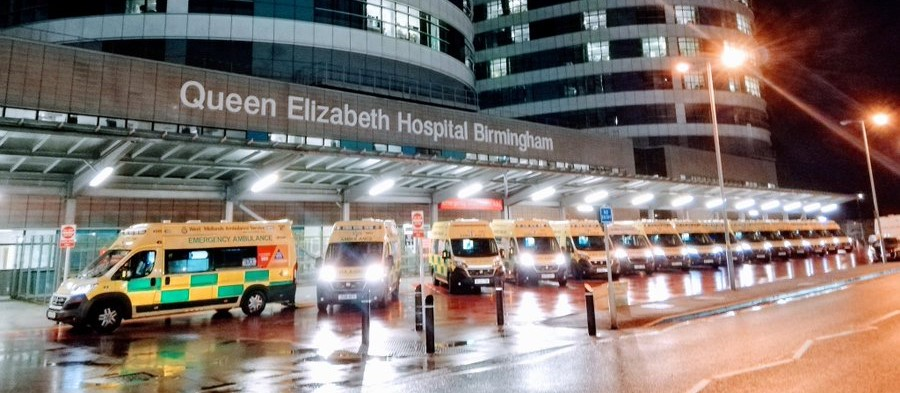
\includegraphics[scale=0.45]{Bin/ambulance_queue.jpg}

\end{frame}

\begin{frame}
    \frametitle{Game - Players}

    \begin{minipage}{.35\textwidth}
        \begin{figure}
            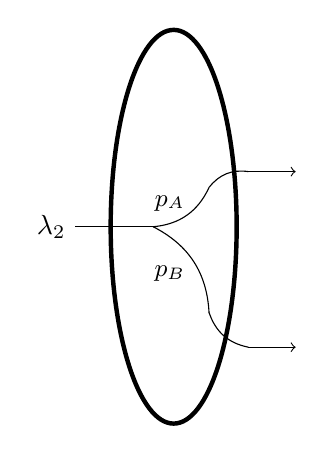
\begin{tikzpicture}
                \draw[ultra thick] (0.75,2) ellipse (0.8cm and 2.5cm);
                % \draw (0,0) -- ++(1.5cm,0) -- ++(0,4cm) -- ++(-1.5cm,0) -- ++ (0, -4cm);
                \draw[-] (0.5, 2) -- ++(-1, 0) node[left] {\(\lambda_2\)};
                
                % p_A line
                \path (0.49, 2) edge [bend right=30] (1.2, 2.5);
                \path (1.2, 2.5) edge [bend left=30] (1.7, 2.7);
                \draw[->] (1.7, 2.7) -- ++(0.6, 0.);
                
                % p_B
                \path (0.49, 2) edge [bend left=30] (1.2, 0.9);
                \path (1.2, 0.91) edge [bend right=30] (1.7, 0.47);
                \draw[->] (1.7, 0.47) -- ++(0.6, 0.);


                \node at (0.7, 2.3) {\small{\( p_A \)}};
                \node at (0.7, 1.4) {\small{\( p_B \)}};

            \end{tikzpicture}
        \end{figure}
    \end{minipage}
    \begin{minipage}{.6\textwidth}
        \begin{figure}
            \scalebox{.8}{
                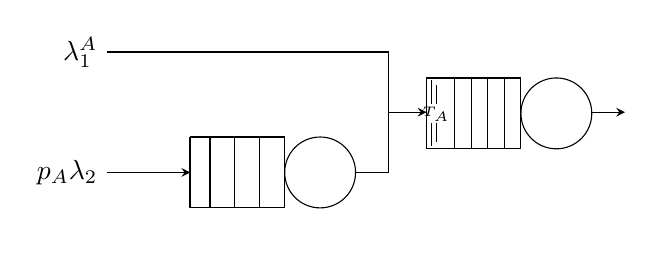
\begin{tikzpicture}[>=stealth, scale=0.6] %arrow type
                    % the rectangle with vertical rules (Queue 1)
                    \draw (0,0) -- ++(2cm,0) -- ++(0,-1.5cm) -- ++(-2cm,0);
                    \foreach \i in {1,...,3, 3.8}
                    \draw (2cm-\i*15pt,0) -- +(0,-1.5cm);
                    
                    % the circle (Queue 1)
                    \draw (2.75,-0.75cm) circle [radius=0.75cm];
            
                    % the rectangle with vertical rules (Queue 2)
                    \draw (5,1.25) -- ++(2cm,0) -- ++(0,-1.5cm) -- ++(-2cm,0);
                    \foreach \i in {1,...,4, 5.7}
                    \draw (7cm-\i*10pt,1.25) -- +(0,-1.5cm);
    
                    % The two vertical lines at the very start of Queue 2 
                    \draw (7cm-54pt,1.2) -- +(0,-0.5cm);
                    \draw (7cm-54pt,0.3) -- +(0,-0.5cm);        
                    \draw (7cm-51pt,1.1) -- +(0,-0.4cm);
                    \draw (7cm-51pt,0.3) -- +(0,-0.4cm);
            
                    % The label between the lines for T
                    \node[anchor=north] at (5.2, 0.84) {\tiny{\( T_A \)}};
    
                    % the circle (Queue 2)
                    \draw (7.75,0.5) circle [radius=0.75cm];
            
                    % the arrows and labels (Queue 1+2)
                    \draw[->] (8.5,0.525) -- +(20pt,0);
                    \node[align=center] at (1cm,-2cm) {};
                    \node[align=center] at (6cm,-0.75cm) {};
                    
                    % Ambulance lines
                    \draw[<-] (0,-0.75) -- +(-50pt,0) node[left] {\( p_A \lambda_2 \)};
                    \draw[-] (3.5,-0.75) -- +(20pt,0);
                    \draw (4.2, 0.525) -- (4.2, -0.75);
    
                    % Others lines
                    \draw (4.2, 1.8) -- +(-169.5pt,0) node[left] {\( \lambda_1^A \)};
                    \draw (4.2, 1.8) -- (4.2, 0.525);
                    \draw[->] (4.2, 0.525) -- (5, 0.525);
                \end{tikzpicture}
            }
            \scalebox{.8}{
                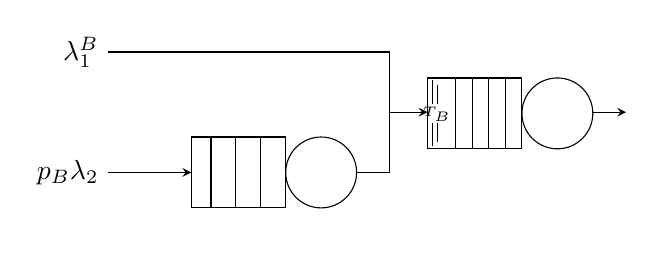
\begin{tikzpicture}[>=stealth, scale=0.6] %arrow type
                    % the rectangle with vertical rules (Queue 1)
                    \draw (0,0) -- ++(2cm,0) -- ++(0,-1.5cm) -- ++(-2cm,0);
                    \foreach \i in {1,...,3, 3.8}
                    \draw (2cm-\i*15pt,0) -- +(0,-1.5cm);
                    
                    % the circle (Queue 1)
                    \draw (2.75,-0.75cm) circle [radius=0.75cm];
            
                    % the rectangle with vertical rules (Queue 2)
                    \draw (5,1.25) -- ++(2cm,0) -- ++(0,-1.5cm) -- ++(-2cm,0);
                    \foreach \i in {1,...,4, 5.7}
                    \draw (7cm-\i*10pt,1.25) -- +(0,-1.5cm);
    
                    % The two vertical lines at the very start of Queue 2 
                    \draw (7cm-54pt,1.2) -- +(0,-0.5cm);
                    \draw (7cm-54pt,0.3) -- +(0,-0.5cm);        
                    \draw (7cm-51pt,1.1) -- +(0,-0.4cm);
                    \draw (7cm-51pt,0.3) -- +(0,-0.4cm);
            
                    % The label between the lines for T
                    \node[anchor=north] at (5.2, 0.84) {\tiny{\( T_B \)}};
    
                    % the circle (Queue 2)
                    \draw (7.75,0.5) circle [radius=0.75cm];
            
                    % the arrows and labels (Queue 1+2)
                    \draw[->] (8.5,0.525) -- +(20pt,0);
                    \node[align=center] at (1cm,-2cm) {};
                    \node[align=center] at (6cm,-0.75cm) {};
                    
                    % Ambulance lines
                    \draw[<-] (0,-0.75) -- +(-50pt,0) node[left] {\( p_B \lambda_2 \)};
                    \draw[-] (3.5,-0.75) -- +(20pt,0);
                    \draw (4.2, 0.525) -- (4.2, -0.75);
    
                    % Others lines
                    \draw (4.2, 1.8) -- +(-169.5pt,0) node[left] {\( \lambda_1^B \)};
                    \draw (4.2, 1.8) -- (4.2, 0.525);
                    \draw[->] (4.2, 0.525) -- (5, 0.525);
                \end{tikzpicture}
            }
        \end{figure}

    \end{minipage}
        
\end{frame}


\begin{frame}
    \frametitle{Game - Strategies}
    \centering

    
\includegraphics[scale=0.1]{Bin/ambulance_cartoon.png}
    \hspace{2cm}
    
\includegraphics[scale=0.1]{Bin/hospital.png}
    \hspace{2cm}
    
\includegraphics[scale=0.1]{Bin/hospital.png}

    \vspace{1cm}
    
\includegraphics[scale=0.2]{Bin/arrows.png}
    \hspace{2cm}
    
\includegraphics[scale=0.04]{Bin/door.png}
    \hspace{2cm}
    
\includegraphics[scale=0.04]{Bin/door.png}

    \[
        p_A, p_B \in [0, 1] \hspace{2cm} T_A \in [1, N_A] \hspace{2cm} T_B \in [1, N_B]
    \]    
    \[
        p_A + p_B = 1 \hspace{8cm}
    \]
\end{frame}
